
% This LaTeX was auto-generated from MATLAB code.
% To make changes, update the MATLAB code and republish this document.

\documentclass{article}
\usepackage{graphicx}
\usepackage{color}

\sloppy
\definecolor{lightgray}{gray}{0.5}
\setlength{\parindent}{0pt}

\begin{document}

    
    
\subsection*{Contents}

\begin{itemize}
\setlength{\itemsep}{-1ex}
   \item Part 1
   \item Part 2
\end{itemize}
\begin{verbatim}
clear;
close all;
clc;
\end{verbatim}


\subsection*{Part 1}

\begin{verbatim}
pep=imread('Assingment 3 Files/peppers.tif');
bab=imread('Assingment 3 Files/baboon.tif');
figure
subplot(3,3,1)
imshow(pep)
for i=1:8
    subplot(3,3,10-i)
    imshow(getBP(pep,i))
end

figure
subplot(3,3,1)
imshow(bab)
for i=1:8
    subplot(3,3,10-i)
    imshow(getBP(bab,i))
end

wmk1=imread('Assingment 3 Files/LSBwmk1.tiff');%2
wmk2=imread('Assingment 3 Files/LSBwmk2.tiff');%1
wmk3=imread('Assingment 3 Files/LSBwmk3.tiff');%1

figure
subplot(2,3,1); imshow(wmk1); title('Original')
subplot(2,3,4); imshow(getBP(wmk1,2)); title('Bit Plane 2')
subplot(2,3,2); imshow(wmk2); title('Original')
subplot(2,3,5); imshow(getBP(wmk2,1)); title('Bit Plane 1')
subplot(2,3,3); imshow(wmk3); title('Original')
subplot(2,3,6); imshow(getBP(wmk3,1)); title('Bit Plane 1')

barb=imread('Assingment 3 Files/Barbara.bmp');
figure
imshow(BPstitch(pep,barb,5))
% figure
% for j=1:8
%     imshow(BPstitch(pep,barb,j))
%     pause
% end

type('getBP.m');
type('BPstitch.m');
\end{verbatim}

        \color{lightgray} \begin{verbatim}
function [bp] = getBP(img,ind)
%UNTITLED3 Summary of this function goes here
%   Detailed explanation goes here
    bp=255*bitget(img,ind);

end


function [encoded] = BPstitch(img,msg,N)
%UNTITLED5 Summary of this function goes here
%   Detailed explanation goes here
    encoded=uint8(zeros(size(img)));
    for i=(N+1):8
        encoded=encoded+(2^(i-1))*bitget(img,i);
    end
    if N==1
        encoded=encoded+bitget(msg,8);
    else
        for i=1:N
            encoded=encoded+(2^(N-i))*bitget(msg,9-i);
        end
    end

    encoded=uint8(encoded);
end

\end{verbatim} \color{black}
    
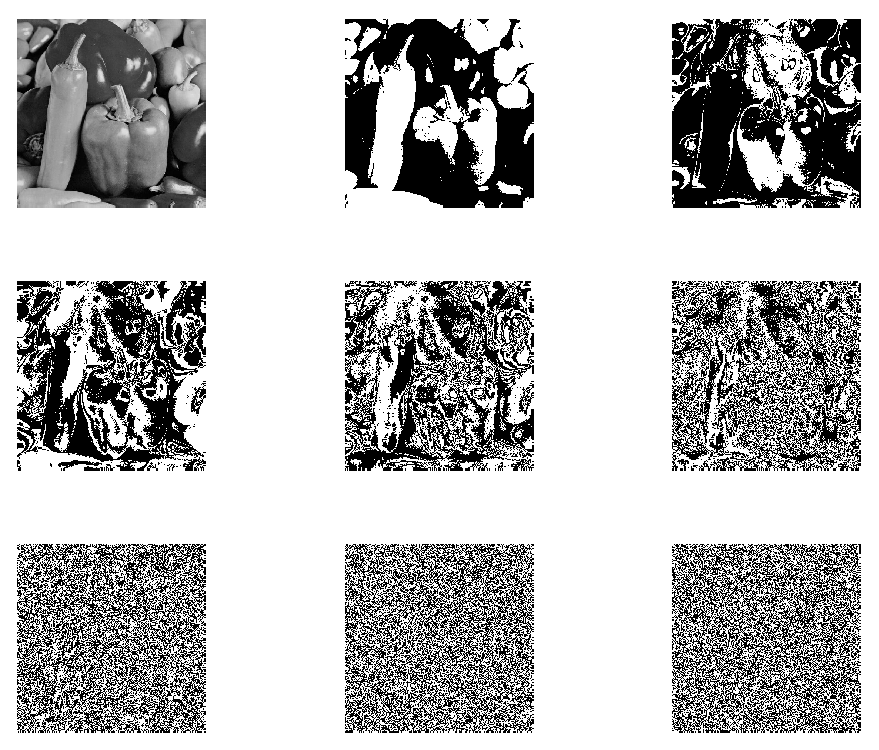
\includegraphics [width=4in]{lab3_01.eps}

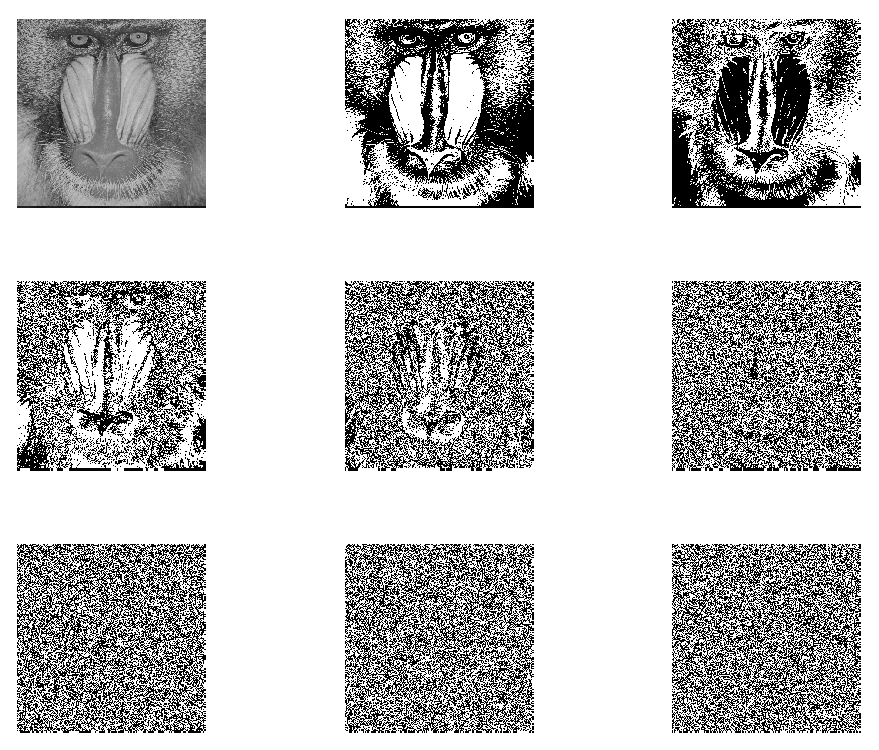
\includegraphics [width=4in]{lab3_02.eps}

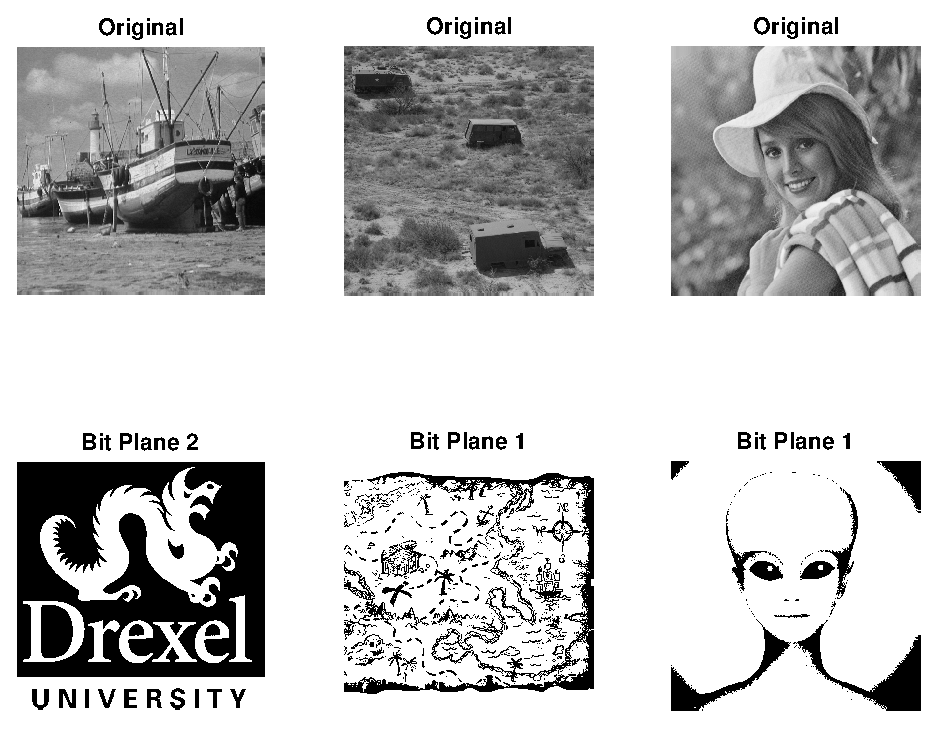
\includegraphics [width=4in]{lab3_03.eps}

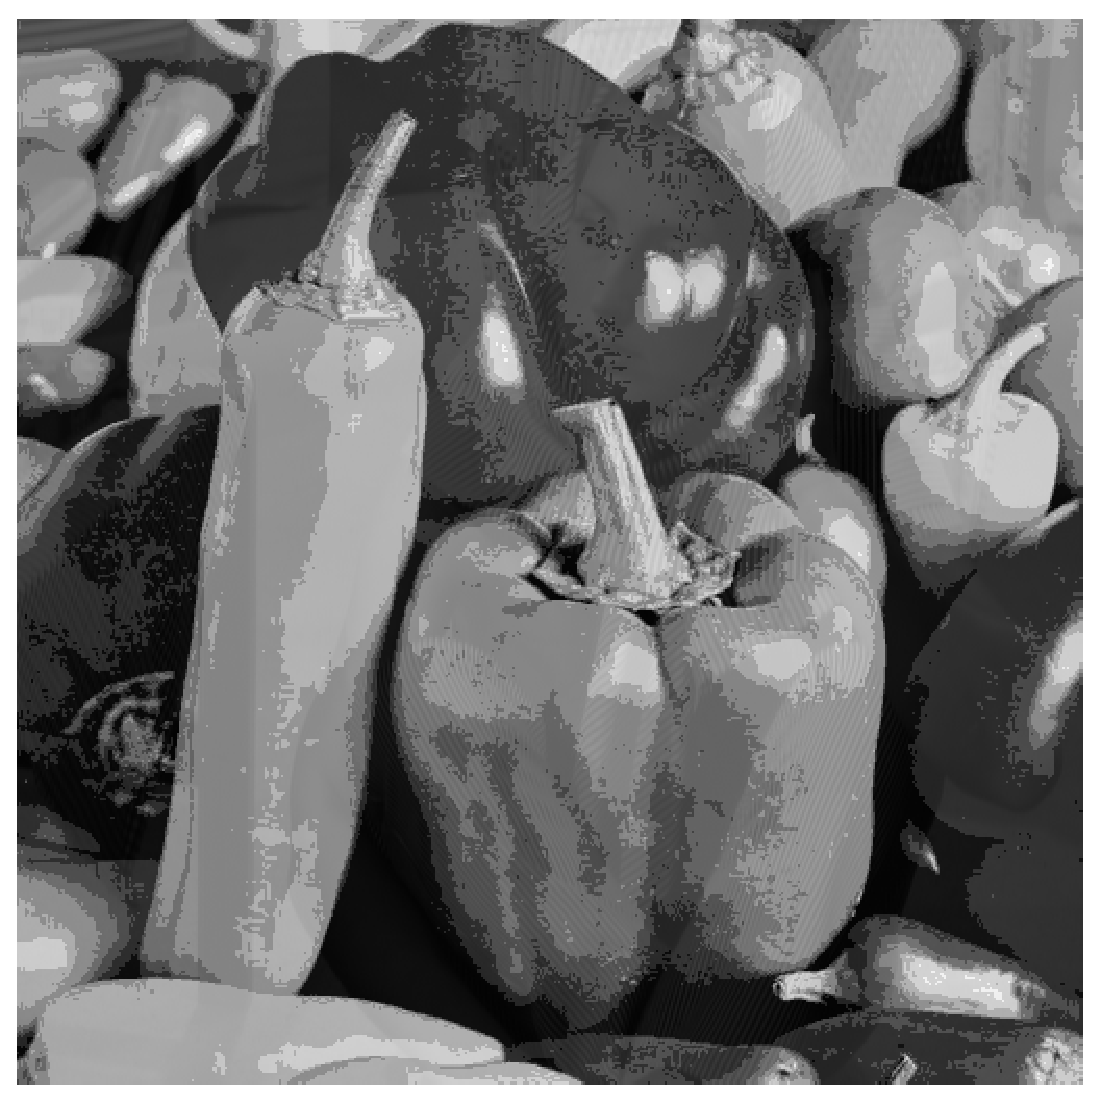
\includegraphics [width=4in]{lab3_04.eps}


\subsection*{Part 2}

\begin{verbatim}
key=256;
wmk=getBP(barb,8)>128;

img1=pep;
[marked1] = YMwatermark( img1,wmk,key );

img2=bab;
[marked2] = YMwatermark( img2,wmk,key );

% see the LSB of marked image
figure
imshow(getBP(marked1,1))
hold on
title('Yeung-Mintzer pepper - Bit plane 1')

figure
imshow(getBP(marked2,1))
hold on
title('Yeung-Mintzer baboon - Bit plane 1')

% get the PSNR
ym_psr_pep=psnr(pep, marked1)
ym_psr_bab=psnr(bab, marked2)

% LSB psnr
lsb_in_pep=BPstitch(pep,barb,1);
lsb_psnr_pep=psnr(pep, lsb_in_pep)

lsb_in_bab=BPstitch(bab,barb,1);
lsb_psnr_bab=psnr(bab, lsb_in_bab)

scrt=imread('Assingment 3 Files/YMwmkedKey435.tiff');
figure
imshow(YMcheck(scrt,435))


manbearpig1=mod(lsb_in_bab,16)+mod(pep,16)*16;
manbearpig2=mod(marked2,16)+mod(pep,16)*16;
figure
subplot(2,2,1)
imshow(manbearpig1)
subplot(2,2,2)
imshow(manbearpig2)
subplot(2,2,3)
imshow(getBP(manbearpig1,1))
subplot(2,2,4)
imshow(YMcheck(manbearpig2,256))
\end{verbatim}

        \color{lightgray} \begin{verbatim}
ym_psr_pep =

   48.2109


ym_psr_bab =

   48.5526


lsb_psnr_pep =

   51.1422


lsb_psnr_bab =

   51.1391

\end{verbatim} \color{black}
    
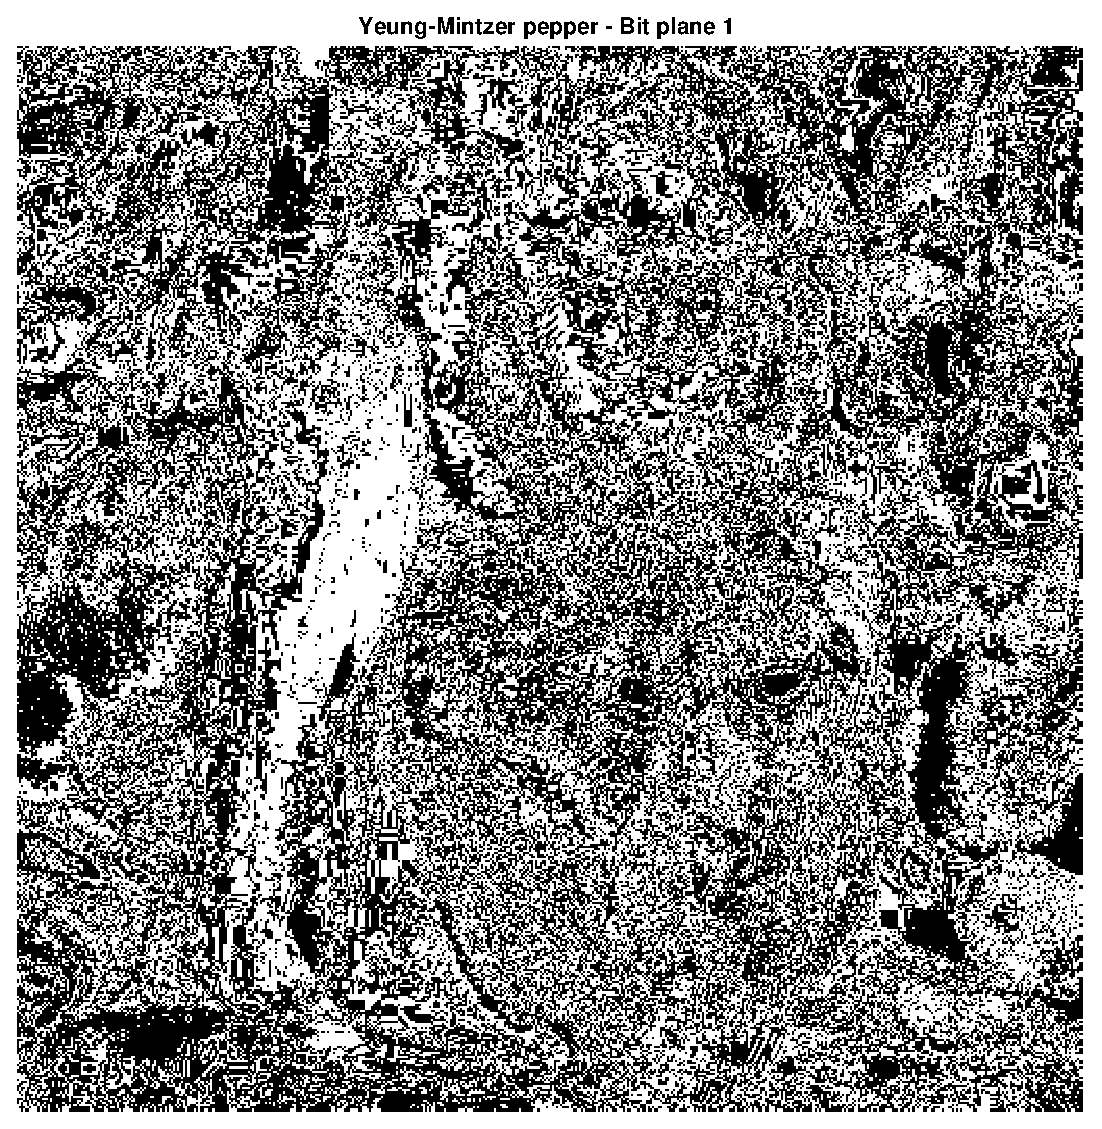
\includegraphics [width=4in]{lab3_05.eps}

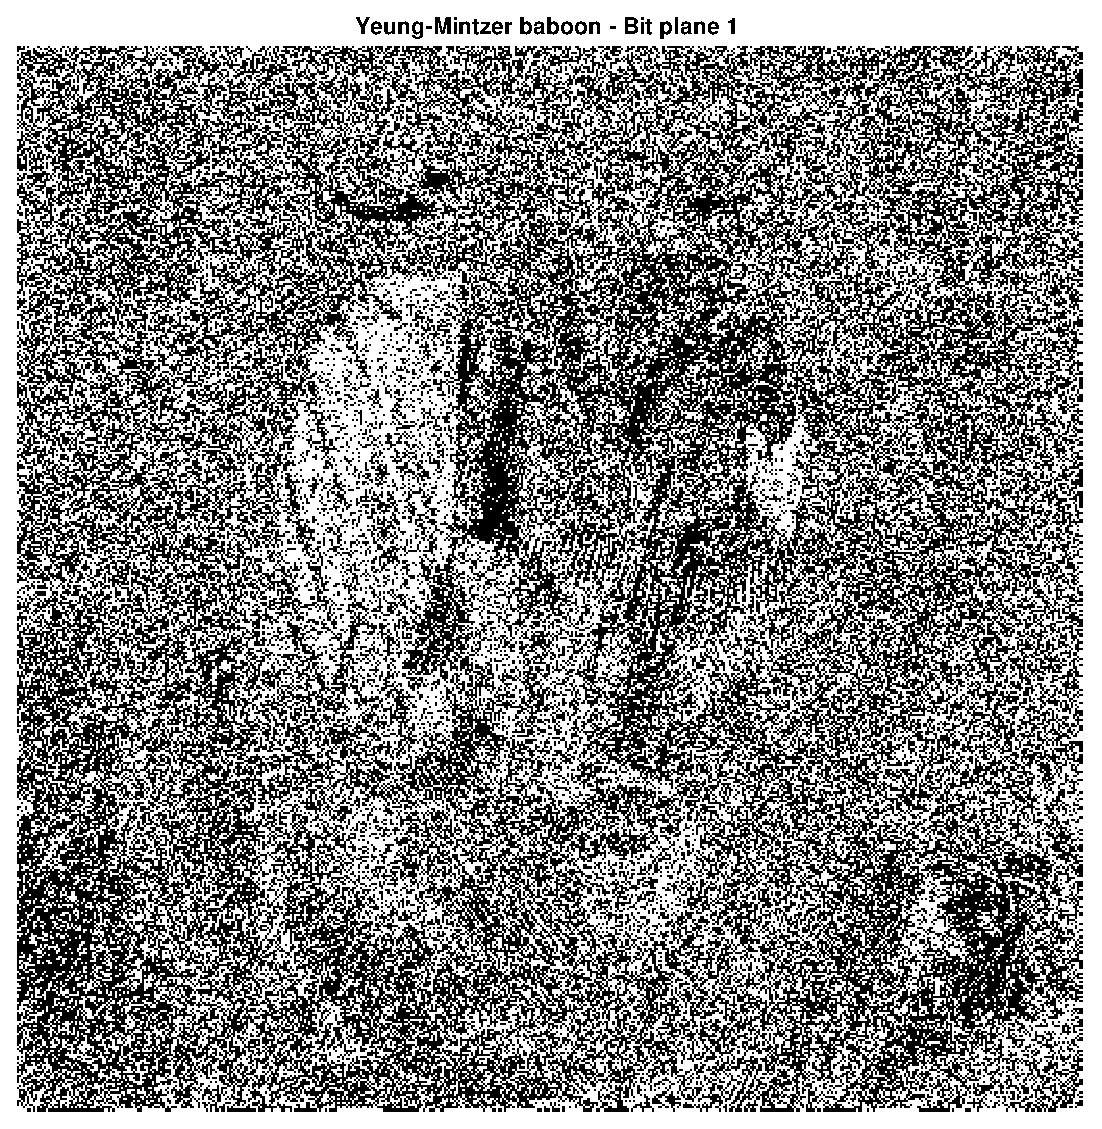
\includegraphics [width=4in]{lab3_06.eps}


\includegraphics [width=4in]{lab3_07.eps}

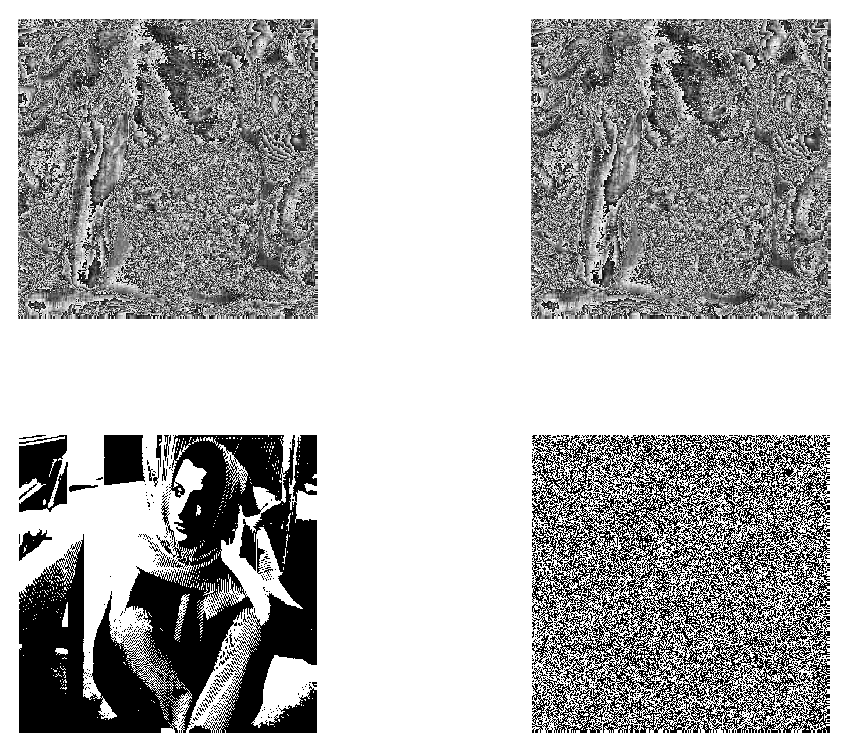
\includegraphics [width=4in]{lab3_08.eps}



\end{document}
    
